% Chapter 2: Literature Review

\chapter{Literature Review}
\label{chap:literature}

\section{Prompt Compression Methodologies}
The escalating cost and latency associated with long-context LLM inference has motivated substantial research into prompt compression. Early techniques focused on abstractive summarization, which utilized smaller auxiliary language models to rewrite source prompts. However, abstractive methods suffer from notable drawbacks: high computational overhead, substantial latency, and the critical risk of hallucinating non-existent facts or omitting granular constraints.

Extractive prompt compression was formalized by Jiang et al.\ with \textbf{LLMLingua} \cite{jiang2023llmlingua}. LLMLingua calculates token perplexity under a compact causal language model (e.g., Llama-2-7B or GPT-2), pruning tokens that exhibit low surprise under the assumption that low-entropy words contribute minimally to core task semantics. While effective on long documents, computing causal perplexities token-by-token remains computationally expensive.

To resolve this latency bottleneck, Pan et al.\ introduced \textbf{LLMLingua-2} \cite{pan2024llmlingua2}. They reformulated prompt compression from causal perplexity calculation into a bidirectional token classification task:
\begin{equation}
    y_i \in \{0, 1\}, \quad \forall t_i \in T
\end{equation}
By distilling compression decisions from GPT-4 on the MeetingBank corpus into an encoder-only Transformer (\texttt{bert-base-multilingual-cased}), LLMLingua-2 achieved 3$\times$--6$\times$ acceleration, allowing compression to run on commodity CPUs. Nonetheless, as demonstrated in this thesis, LLMLingua-2 was trained exclusively on clean English meeting transcripts and lacks domain adaptation for transliterated, informal code-mixed text.

\section{Code-Mixed Natural Language Processing}
Code-mixing—the alternating use of two or more languages within a single utterance—is prevalent across South Asian digital communication. Romanized Hindi-English (Hinglish) introduces severe natural language understanding bottlenecks:
\begin{enumerate}
    \item \textbf{Spelling Entropy (Orthographic Chaos):} Because Romanized Hindi lacks standardized spelling, phonetic variants proliferate widely (e.g., \textit{``kyu''}, \textit{``kyun''}, \textit{``kew''}, \textit{``q''} for the Hindi word \textit{क्यों} / \textit{why}).
    \item \textbf{Phonetic and Morphological Affixation:} Hindi verb conjugations frequently fuse with English root nouns (e.g., \textit{``schedule-karna''}, \textit{``cancel-ho-gaya''}).
    \item \textbf{High Density of Function Words and Fillers:} Conversational Hinglish discourse features frequent discourse markers (e.g., \textit{``yaar''}, \textit{``matlab''}, \textit{``arre''}, \textit{``toh''}) that inflate token counts without contributing propositional content.
\end{enumerate}

Petrov et al.\ \cite{petrov2023language} quantified tokenizer unfairness across 100+ languages, documenting that subword algorithms (such as SentencePiece and WordPiece) create massive token inflation on non-English text. While specialized Indian language models such as MuRIL \cite{khanuja2021muril} and benchmarks like GLUECoS \cite{khanuja2020gluecos} and PRESTO \cite{goel2023presto} have addressed classification and parsing, no prior literature has systematically measured the survival of code-mixed dialogue under lossy extractive prompt compression.

\section{LLM Cascade Routing}
Model cascading is an established strategy to minimize inference expenditure by routing requests between heterogeneous model tiers. \textbf{FrugalGPT} \cite{chen2023frugalgpt} demonstrated that a sequential cascade of API calls—querying cheaper models first and falling back to GPT-4 upon failure—drastically reduces operational costs. \textbf{RouteLLM} \cite{ong2024routellm} extended this concept by training learned preference routers (using matrix factorization and classifier heads) to predict whether an 8B model will achieve human-preferred answers over a 70B model.

However, existing cascade routers operate predominantly on heuristic thresholds or soft probability scores, lacking distribution-free statistical guarantees against catastrophic failure on high-complexity tasks.

\section{Conformal Prediction and Risk Control}
Conformal prediction, pioneered by Vovk et al.\ and formalized for modern machine learning by Angelopoulos and Bates \cite{angelopoulos2021gentle}, offers a rigorous framework for distribution-free uncertainty quantification. 

\begin{figure}[htbp]
    \centering
    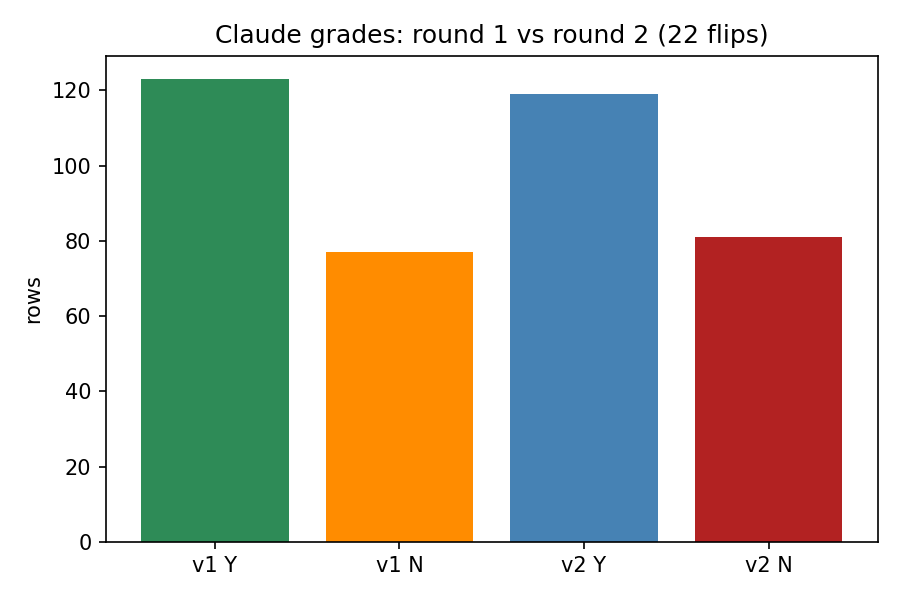
\includegraphics[width=0.85\linewidth]{Figures/fig_grades.png}
    \caption{Distribution of automated and blinded expert grades across difficulty splits in the router evaluation pipeline.}
    \label{fig:grades_distribution}
\end{figure}

In the context of risk-controlled cascade routing, the \textbf{Learn-Then-Test (LTT)} framework \cite{angelopoulos2024conformal} allows an operator to select a routing threshold $\tau^*$ such that the expected risk (the probability of cheap-model failure) remains bounded below a pre-specified tolerance $\alpha$:
\begin{equation}
    \mathbb{P}\Big( R(\tau^*) \le \alpha \Big) \ge 1 - \delta
\end{equation}
where $R(\tau)$ denotes the empirical risk evaluated over a finite calibration split, and $\delta$ denotes the statistical confidence level (e.g., $\delta = 0.05$).

\section{Identified Research Gaps}
Our review reveals four critical deficiencies in the existing state-of-the-art:
\begin{itemize}
    \item \textbf{Monolingual Bias:} Published prompt compression benchmarks (MeetingBank, GSM8K, LongBench) focus almost exclusively on standard English.
    \item \textbf{Entity Mangling Blindspot:} Neither LLMLingua nor LLMLingua-2 measures or enforces the survival of structured entities (emails, timestamps, monetary amounts, phone numbers) after compression.
    \item \textbf{Absence of Statistical Guarantees in Routing:} Current model routers rely on uncalibrated confidence scores without provable risk bounds.
    \item \textbf{Decoupled Architectures:} Prior works evaluate prompt compression and model routing in complete isolation, ignoring the strong compounding economic benefits of combining both within a single serving gateway.
\end{itemize}
